%%%%%%%%%%%%%%%%%%%%%%%%%%%%%%%%%%%%%%%%%
% Short Sectioned Assignment
% LaTeX Template
% Version 1.0 (5/5/12)
%
% This template has been downloaded from:
% http://www.LaTeXTemplates.com
%
% Original author:
% Frits Wenneker (http://www.howtotex.com)
%
% License:
% CC BY-NC-SA 3.0 (http://creativecommons.org/licenses/by-nc-sa/3.0/)
%
%%%%%%%%%%%%%%%%%%%%%%%%%%%%%%%%%%%%%%%%%

%----------------------------------------------------------------------------------------
%	PACKAGES AND OTHER DOCUMENT CONFIGURATIONS
%----------------------------------------------------------------------------------------

\documentclass[paper=a4, fontsize=11pt]{scrartcl} % A4 paper and 11pt font size

\usepackage[T1]{fontenc} % Use 8-bit encoding that has 256 glyphs
%\usepackage{fourier} % Use the Adobe Utopia font for the document - comment this line to return to the LaTeX default
\usepackage[english]{babel} % English language/hyphenation
\usepackage{amsmath,amsfonts,amsthm} % Math packages
\usepackage{bm}
\usepackage{lipsum} % Used for inserting dummy 'Lorem ipsum' text into the template
\usepackage{graphicx} % This one is for pictures
\usepackage{sectsty} % Allows customizing section commands
\allsectionsfont{\centering \normalfont\scshape} % Make all sections centered, the default font and small caps

\usepackage{fancyhdr} % Custom headers and footers
\pagestyle{fancyplain} % Makes all pages in the document conform to the custom headers and footers
\fancyhead{} % No page header - if you want one, create it in the same way as the footers below
\fancyfoot[L]{} % Empty left footer
\fancyfoot[C]{} % Empty center footer
\fancyfoot[R]{\thepage} % Page numbering for right footer
\renewcommand{\headrulewidth}{0pt} % Remove header underlines
\renewcommand{\footrulewidth}{0pt} % Remove footer underlines
\setlength{\headheight}{13.6pt} % Customize the height of the header

\numberwithin{equation}{section} % Number equations within sections (i.e. 1.1, 1.2, 2.1, 2.2 instead of 1, 2, 3, 4)
\numberwithin{figure}{section} % Number figures within sections (i.e. 1.1, 1.2, 2.1, 2.2 instead of 1, 2, 3, 4)
\numberwithin{table}{section} % Number tables within sections (i.e. 1.1, 1.2, 2.1, 2.2 instead of 1, 2, 3, 4)

\setlength\parindent{0pt} % Removes all indentation from paragraphs - comment this line for an assignment with lots of text

%----------------------------------------------------------------------------------------
%	TITLE SECTION
%----------------------------------------------------------------------------------------

\newcommand{\horrule}[1]{\rule{\linewidth}{#1}} % Create horizontal rule command with 1 argument of height

\title{	
\normalfont \normalsize 
\textsc{Columbia University -- Fall 2013} \\ [25pt] % Your university, school and/or department name(s)
\horrule{0.5pt} \\[0.4cm] % Thin top horizontal rule
\huge Machine Learning Homework \#1\\ % The assignment title
\horrule{2pt} \\[0.5cm] % Thick bottom horizontal rule
}

\author{Joe Ellis} % Your name

\date{\normalsize\today} % Today's date or a custom date

\begin{document}

\maketitle % Print the title

%----------------------------------------------------------------------------------------
%	PROBLEM 1
%----------------------------------------------------------------------------------------

\section{Problem 1}

In this problem we investigate fitting a polynomial model and regression to a dataset consiting of 10 data points.  
Our $d$-dimensional polynomail function, $f$, is described below, 

\begin{align} 
f(x;\bm{\theta}) = \bm{\theta}_{0}	+ \bm{\theta}_{1}x_{1} + \bm{\theta}_{2}x_{2} + ... + \bm{\theta}_{d}x_{d}		
\end{align}

where $\bm{\theta}$ is the learned parameters of our model, and $x$ is a given data point.
We choose to use squared error for our empirical loss function to gauge how well our model fits the data present.  The equation for empirical loss can be seen below, where $x$ represents the given data points, $y$ represents the output, which our function $f$ is attempting to solve for.

\begin{align} 
R_{emp}(\bm{\theta}) = \frac{1}{N}\sum\limits_{i=1}^n (y_{i} - f(x_{i};\bm{\theta}))^{2}
\end{align}

We perform cross-validation to find the adequate dimensionality of an appropriate model.  
The cross-validation performed is completed 1000 times for each model complexity with train/test split of 9 points for training and 1 point for testing.  The results of the cross-validation can be seen in Figure 1., and we can see that a model of 4 or 5 dimesions is suitable for this dataset.  Models with lower than 3-dimensions have a hard time describing the variation in the data, where as models with many more than 3-dimensions tend to overfit.

\begin{figure}
\centering
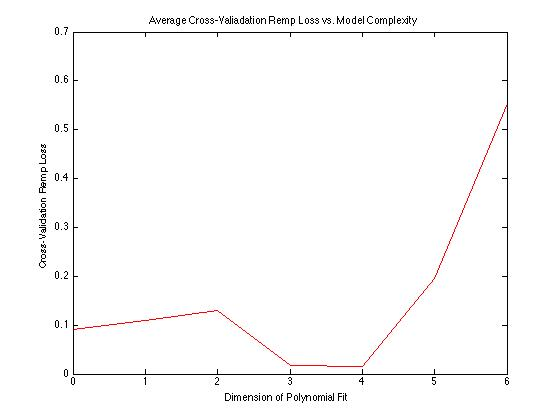
\includegraphics[scale=0.5]{Prob1_CrossValError.jpg}
\end{figure}

Using the 3-dimensional model for $f$ we achieve the best polynomial regression function with, 

\begin{align} 
\bm{\theta} = [0.1951 5.4884 -19.6041 
\end{align}


%------------------------------------------------

\subsection{Heading on level 2 (subsection)}

Lorem ipsum dolor sit amet, consectetuer adipiscing elit. 
\begin{align}
A = 
\begin{bmatrix}
A_{11} & A_{21} \\
A_{21} & A_{22}
\end{bmatrix}
\end{align}
Aenean commodo ligula eget dolor. Aenean massa. Cum sociis natoque penatibus et magnis dis parturient montes, nascetur ridiculus mus. Donec quam felis, ultricies nec, pellentesque eu, pretium quis, sem.

%------------------------------------------------

\subsubsection{Heading on level 3 (subsubsection)}

\lipsum[3] % Dummy text

\paragraph{Heading on level 4 (paragraph)}

\lipsum[6] % Dummy text

%----------------------------------------------------------------------------------------
%	PROBLEM 2
%----------------------------------------------------------------------------------------

\section{Lists}

%------------------------------------------------

\subsection{Example of list (3*itemize)}
\begin{itemize}
	\item First item in a list 
		\begin{itemize}
		\item First item in a list 
			\begin{itemize}
			\item First item in a list 
			\item Second item in a list 
			\end{itemize}
		\item Second item in a list 
		\end{itemize}
	\item Second item in a list 
\end{itemize}

%------------------------------------------------

\subsection{Example of list (enumerate)}
\begin{enumerate}
\item First item in a list 
\item Second item in a list 
\item Third item in a list
\end{enumerate}

%----------------------------------------------------------------------------------------

\end{document}